\documentclass{ip-quiz}

\quizlevel{n1}
\quiznum{2}
\quiztitle{Funciones - Opción 0}

\begin{document}

\makeheader
\maketitle

\begin{sectionbox}{Enunciado}
Considere un cuadrado inscrito en un círculo de radio $r$. Los vértices del cuadrado tocan la circunferencia.

\begin{center}
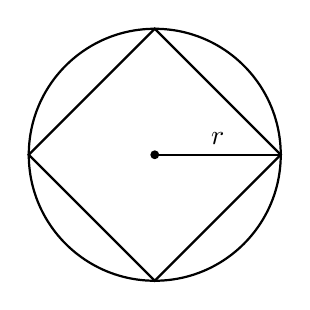
\begin{tikzpicture}[scale=0.8]
    % Circle
    \draw[thick] (2,2) circle (2);
    
    % Square inscribed (rotated 45 degrees, vertices on circle)
    \draw[thick] (2,0) -- (4,2) -- (2,4) -- (0,2) -- cycle;
    
    % Radius line
    \draw[thick] (2,2) -- (4,2);
    \fill (2,2) circle (2pt);
    
    % Radius label
    \node[above] at (3,2) {$r$};
\end{tikzpicture}
\end{center}

Defina una función llamada \texttt{calcular\_area\_cuadrado} que reciba como parámetro el radio $r$ del círculo y retorne el área del cuadrado.
\end{sectionbox}

\begin{sectionbox}{Solución}
\begin{minted}{python}
def calcular_area_cuadrado(r: float) -> float:
    diagonal_del_cuadrado = 2 * r
    hipotenusa_al_cuadrado = diagonal_del_cuadrado ** 2
    cateto_al_cuadrado = hipotenusa_al_cuadrado / 2
    return cateto_al_cuadrado  # El cateto es el lado; al cuadrado, es el área.
\end{minted}
\end{sectionbox}

\end{document}